\documentclass[journal,12pt,twocolumn]{IEEEtran}
%

\usepackage{setspace}
\usepackage{gensymb}
\singlespacing

\usepackage{amsmath}
\usepackage{amsthm}
\usepackage{txfonts}
\usepackage{cite}
\usepackage{enumitem}
\usepackage{mathtools}
\usepackage{listings}
    \usepackage{color}                                            %%
    \usepackage{array}                                            %%
    \usepackage{longtable}                                        %%
    \usepackage{calc}                                             %%
    \usepackage{multirow}                                         %%
    \usepackage{hhline}                                           %%
    \usepackage{ifthen}                                           %%
  %optionally (for landscape tables embedded in another document): %%
    \usepackage{lscape}     
\usepackage{multicol}
\usepackage{chngcntr}
\usepackage{tikz}
\usepackage{pgfplots}
\usepackage{gensymb}
\renewcommand\thesection{\arabic{section}}
\renewcommand\thesubsection{\thesection.\arabic{subsection}}
\renewcommand\thesubsubsection{\thesubsection.\arabic{subsubsection}}

\renewcommand\thesectiondis{\arabic{section}}
\renewcommand\thesubsectiondis{\thesectiondis.\arabic{subsection}}
\renewcommand\thesubsubsectiondis{\thesubsectiondis.\arabic{subsubsection}}

% correct bad hyphenation here
\hyphenation{op-tical net-works semi-conduc-tor}
\def\inputGnumericTable{}                                 %%

\lstset{
%language=C,
frame=single, 
breaklines=true,
columns=fullflexible
}
\begin{document}
%
\newtheorem{theorem}{Theorem}[section]
\newtheorem{problem}{Problem}
\newtheorem{proposition}{Proposition}[section]
\newtheorem{lemma}{Lemma}[section]
\newtheorem{corollary}[theorem]{Corollary}
\newtheorem{example}{Example}[section]
\newtheorem{definition}[problem]{Definition}
\newcommand{\BEQA}{\begin{eqnarray}}
\newcommand{\EEQA}{\end{eqnarray}}
\newcommand{\define}{\stackrel{\triangle}{=}}
\bibliographystyle{IEEEtran}
\providecommand{\mbf}{\mathbf}
\providecommand{\pr}[1]{\ensuremath{\Pr\left(#1\right)}}
\providecommand{\qfunc}[1]{\ensuremath{Q\left(#1\right)}}
\providecommand{\sbrak}[1]{\ensuremath{{}\left[#1\right]}}
\providecommand{\lsbrak}[1]{\ensuremath{{}\left[#1\right.}}
\providecommand{\rsbrak}[1]{\ensuremath{{}\left.#1\right]}}
\providecommand{\brak}[1]{\ensuremath{\left(#1\right)}}
\providecommand{\lbrak}[1]{\ensuremath{\left(#1\right.}}
\providecommand{\rbrak}[1]{\ensuremath{\left.#1\right)}}
\providecommand{\cbrak}[1]{\ensuremath{\left\{#1\right\}}}
\providecommand{\lcbrak}[1]{\ensuremath{\left\{#1\right.}}
\providecommand{\rcbrak}[1]{\ensuremath{\left.#1\right\}}}
\theoremstyle{remark}
\newtheorem{rem}{Remark}
\newcommand{\sgn}{\mathop{\mathrm{sgn}}}
\providecommand{\abs}[1]{\left\vert#1\right\vert}
\providecommand{\res}[1]{\Res\displaylimits_{#1}} 
\providecommand{\norm}[1]{\left\lVert#1\right\rVert}
\providecommand{\mtx}[1]{\mathbf{#1}}
\providecommand{\mean}[1]{E\left[ #1 \right]}
\providecommand{\fourier}{\overset{\mathcal{F}}{ \rightleftharpoons}}
\providecommand{\system}{\overset{\mathcal{H}}{ \longleftrightarrow}}
\newcommand{\solution}{\noindent \textbf{Solution: }}
\newcommand{\cosec}{\,\text{cosec}\,}
\providecommand{\dec}[2]{\ensuremath{\overset{#1}{\underset{#2}{\gtrless}}}}
\newcommand{\myvec}[1]{\ensuremath{\begin{pmatrix}#1\end{pmatrix}}}
\newcommand{\cmyvec}[1]{\ensuremath{\begin{pmatrix*}[c]#1\end{pmatrix*}}}
\newcommand{\mydet}[1]{\ensuremath{\begin{vmatrix}#1\end{vmatrix}}}
\newcommand{\proj}[2]{\textbf{proj}_{\vec{#1}}\vec{#2}}
\let\StandardTheFigure\thefigure
\let\vec\mathbf
\title{Assignment - 3}
\author{Padmanabh
\\ MD/2020/708}
% make the title area
\maketitle
\newpage
%\tableofcontents
\bigskip
\renewcommand{\thefigure}{\theenumi}
\renewcommand{\thetable}{\theenumi}
%\renewcommand{\theequation}{\theenumi}
%Download all python codes 
%
%\begin{lstlisting}
%svn co https://github.com/JayatiD93/trunk/My_solution_design/codes
%\end{lstlisting}
Download all and latex-tikz codes from 
%
\begin{lstlisting}
svn co https://github.com/Padmanabhk1/Assignment-3.git
\end{lstlisting}
%
%
Question taken from
\begin{lstlisting}
https://github.com/gadepall/ncert/blob/main/linalg/construction/gvv_ncert_constr.pdf- example 2.7
\end{lstlisting}
%
    
\section{Question}
Construct a quadrilateral MIST where $MI = 3.5, IS = 6.5, \angle M = 75\degree , \angle I = 105\degree$ and $\angle S = 120\degree$
\section{solution}
The basic property of quadrilateral is that-
\begin{enumerate}
\begin{lemma}
     \item A quadrilateral should be closed shape with 4 sides
\end{lemma}
\begin{lemma}
     \item All the internal angles of a quadrilateral sum up to 360°
\end{lemma}
\end{enumerate}

Let us consider first case, Where quadrilateral MIST has is constructed considering following parameters\\
\begin{align}
   $MI = 3.5 cm,$\\ 
$IS = 6.5 cm,$\\
\angle M = 75\degree,\\\
\angle I = 105\degree\\
\angle S = 120\degree 
\end{align}

The quadrilateral was plotted with given parameters,
Co-ordinates were found to be-

$$\vec {M} =\myvec {0\\0}\\$$
$$\vec {I} =\myvec {5\\0}\\$$
$$\vec {S} =\myvec {7.3\\6.3}\\$$
$$\vec {T} =\myvec {2.5\\5.4}\\$$
Based on the co-ordinates, The value of angle T was calculated
$$\angle T = 55\degree$$
Now, The sum of all angles should be 360\degree
if MIST is a quadrilateral,
Then
$$\angle M+\angle I+\angle S+\angle T= 360\degree$$
75+110+120+55 = 360\degree\\
Thus, The figure plotted with given parameters fulfills the criterion, i.e the sum of angles of a quadrilateral should be 360\degree , Thus we can plot the quadrilateral with given parameters.\\

\begin{figure}[assignment 3.png]
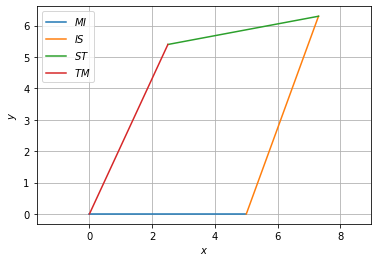
\includegraphics[width=\columnwidth]{assignment 3.png}
  \caption{Quadrilateral MIST when \angle M=75}
  \label{fig:Quadrilateral MIST}
\end{figure}
\end{document}